\FloatBarrier
\section{Multiplicity Distributions}

Previous measurements of two particle correlations have been done at hadron collider experiments, such as CMS.  These measurements typically are typically done in bins of event multiplicity in order to quantify the activity in a set of events.  Because ALEPH has a different acceptance than the CMS detector, and because $e^{+}e^{-}$ collisions have different kinematics than those at hadron colliders, some conversion needs to be done in order to compare events of a given multiplicity in ALEPH with those in CMS.  For the studies done here, we require charged tracks to have $p_{T}<0.2$ GeV and $|\eta|<1.8$ in ALEPH, and $p_{T}<0.4$ and $|\eta|<2.4$ in CMS.  The latter requirement is identical to the cuts used in all CMS papers on two particle correlations.  The multiplicity distribution in LEP1 ALEPH events can be seen in Fig.~\ref{fig:LEP1Mult}.  The tracking efficiency as a function of event multiplicity can be seen in Fig.~\ref{fig:LEP1Eff}, calculated by matching reconstructed tracks to generator-level particles in ALEPH Monte Carlo.  The dip at low multiplicity is most likely due to a self-bias causing low-efficiency events to also have low multiplicity.  After taking into account both the efficiency and acceptance of the ALEPH detector, the total fraction of charged particles reconstructed is shown in Fig.~\ref{fig:LEP1EffAccept}.  In the highest multiplcity events, the ALEPH detector reconstructions around 50\% of all the charged particles in an event.

The acceptance of the CMS detector, as calculated by seeing how many generator-level charged particles pass the
$\eta$ cut, in pp pythia Monte Carlo events is shown in Fig.~\ref{fig:CMSAcc}.  This is done as a function of generator-level multiplicity.  Roughly 30\% of all charged particles can be reconstructed in CMS for pp collisions.  Using Fig.~\ref{fig:LEP1EffAccept} and Fig.~\ref{fig:CMSAcc}, a conversion factor can be calculated to convert the reconstructed ALEPH multiplicity to an equivilent corrected multiplicity for a hadron collider.  This conversion factor is shown in Fig.~\ref{fig:conversion}, and the mapping from ALEPH multiplicities to CMS multiplicities is shown in Fig.~\ref{fig:conversion2}.  The behavior at low multiplicities is caused by the self-bias of the efficiency and acceptances with the multiplicity calculation.  However, this analysis is mostly interested in events having high multiplicity, where the conversion factor converges to a reasonable factor of around 0.7.  After applying this mapping to the distribution in Fig.~\ref{fig:LEP1Mult}, the multiplicity distribution that can be used for comparing with CMS results is shown in Fig.~\ref{fig:CMSComparison}.

\begin{figure}[!htb]
\begin{center}
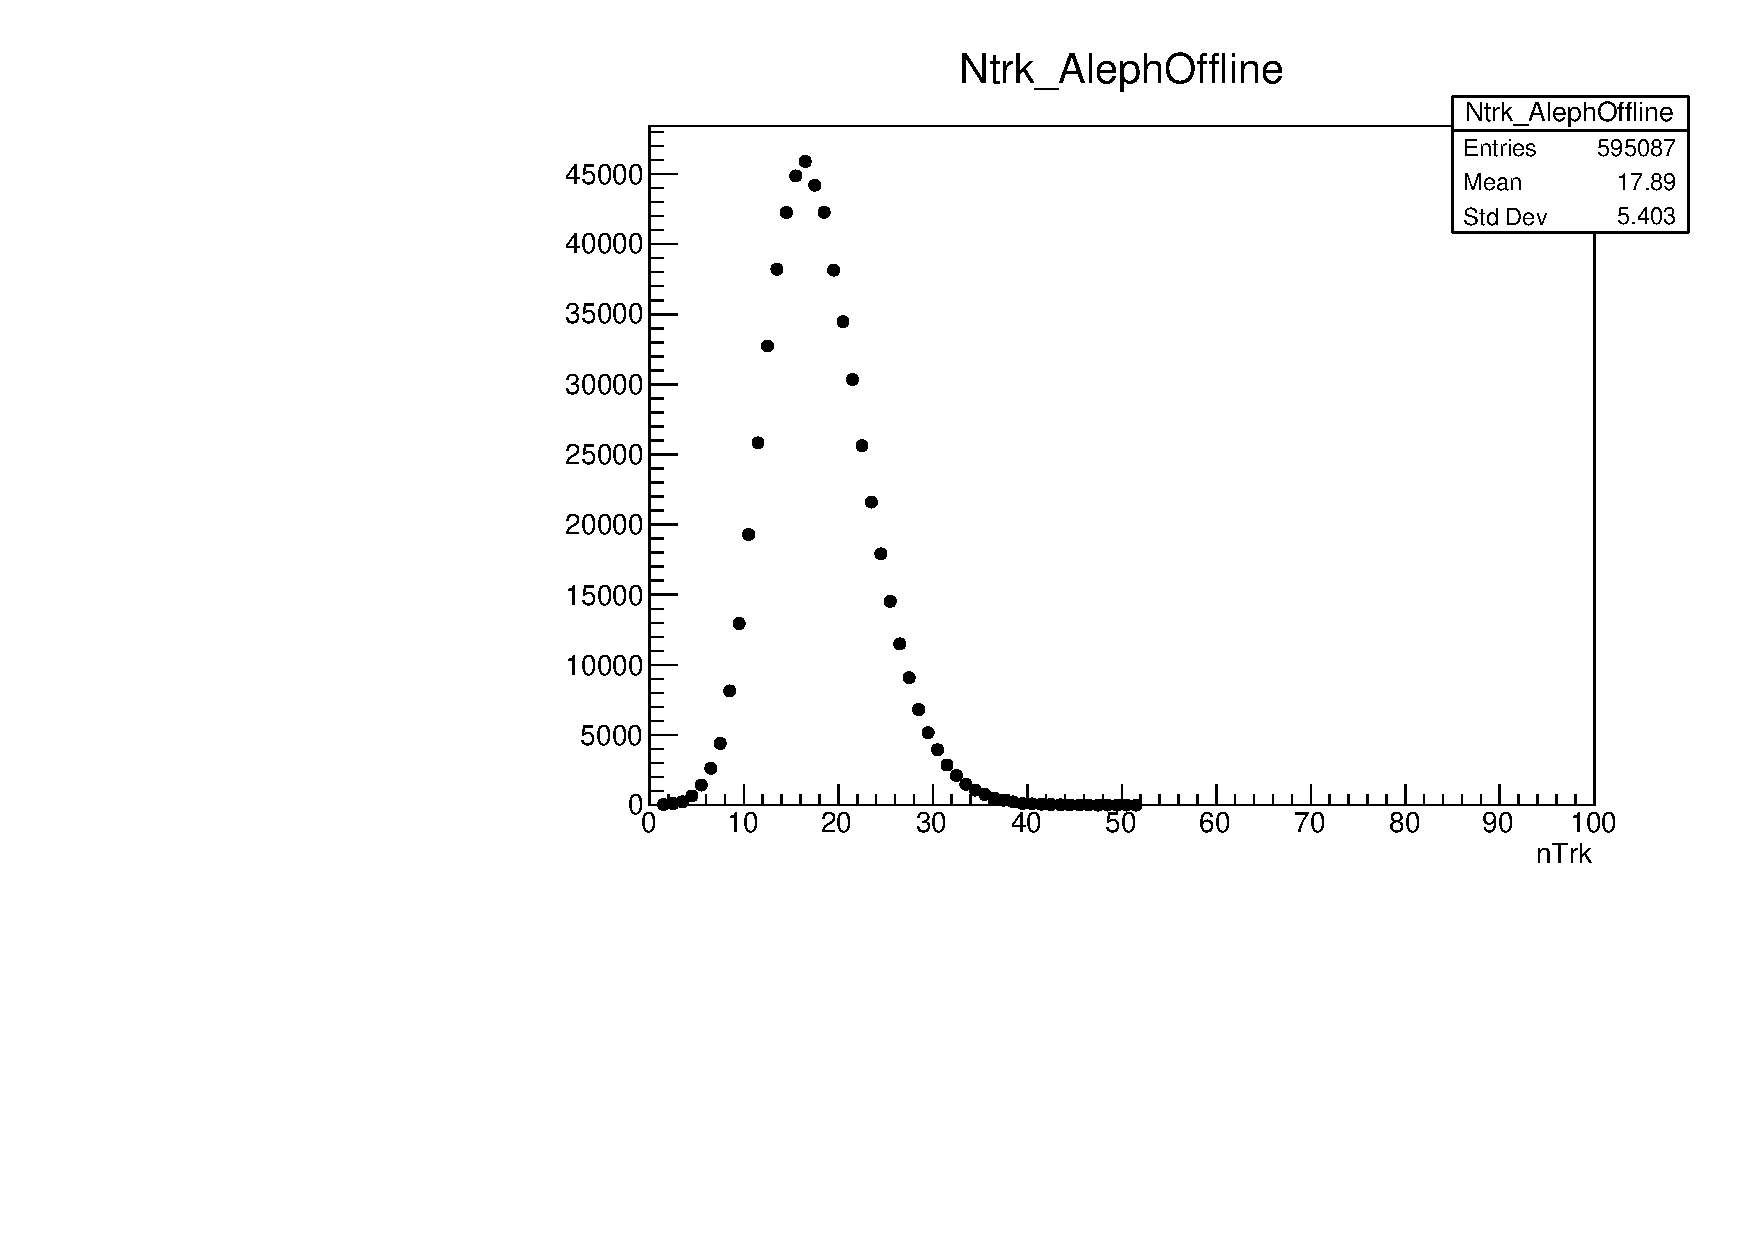
\includegraphics[width=.45\textwidth]{images/MultiplicityConversion/nTrkOffline_ALEPH.pdf}
\caption{LEP1 Multiplicity Distribution}
\label{fig:LEP1Mult} 
\end{center}
\end{figure}

\begin{figure}[!htb]
\begin{center}
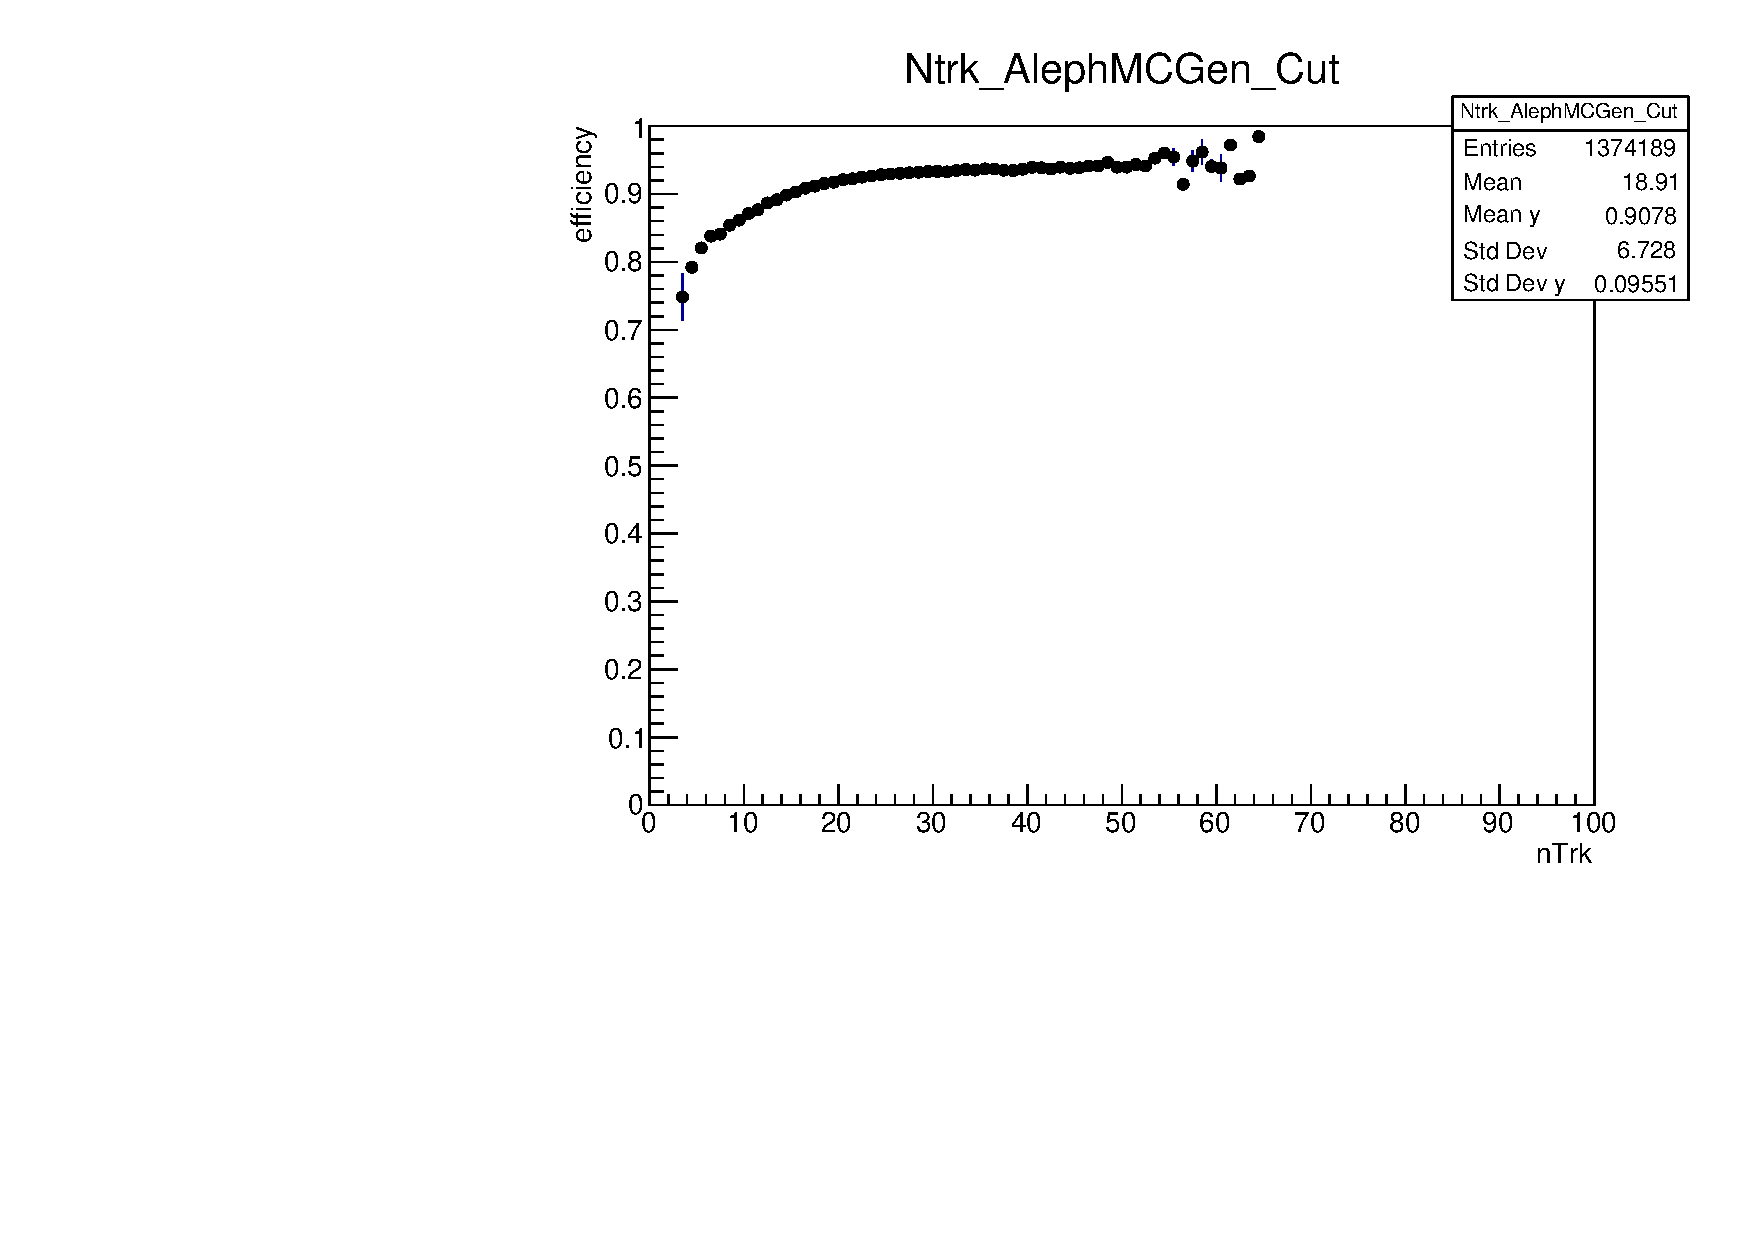
\includegraphics[width=.45\textwidth]{images/MultiplicityConversion/nTrk_AlephMCGen_Cut.pdf}
\caption{LEP1 Efficiency Distribution vs Multiplcity}
\label{fig:LEP1Eff} 
\end{center}
\end{figure}

\begin{figure}[!htb]
\begin{center}
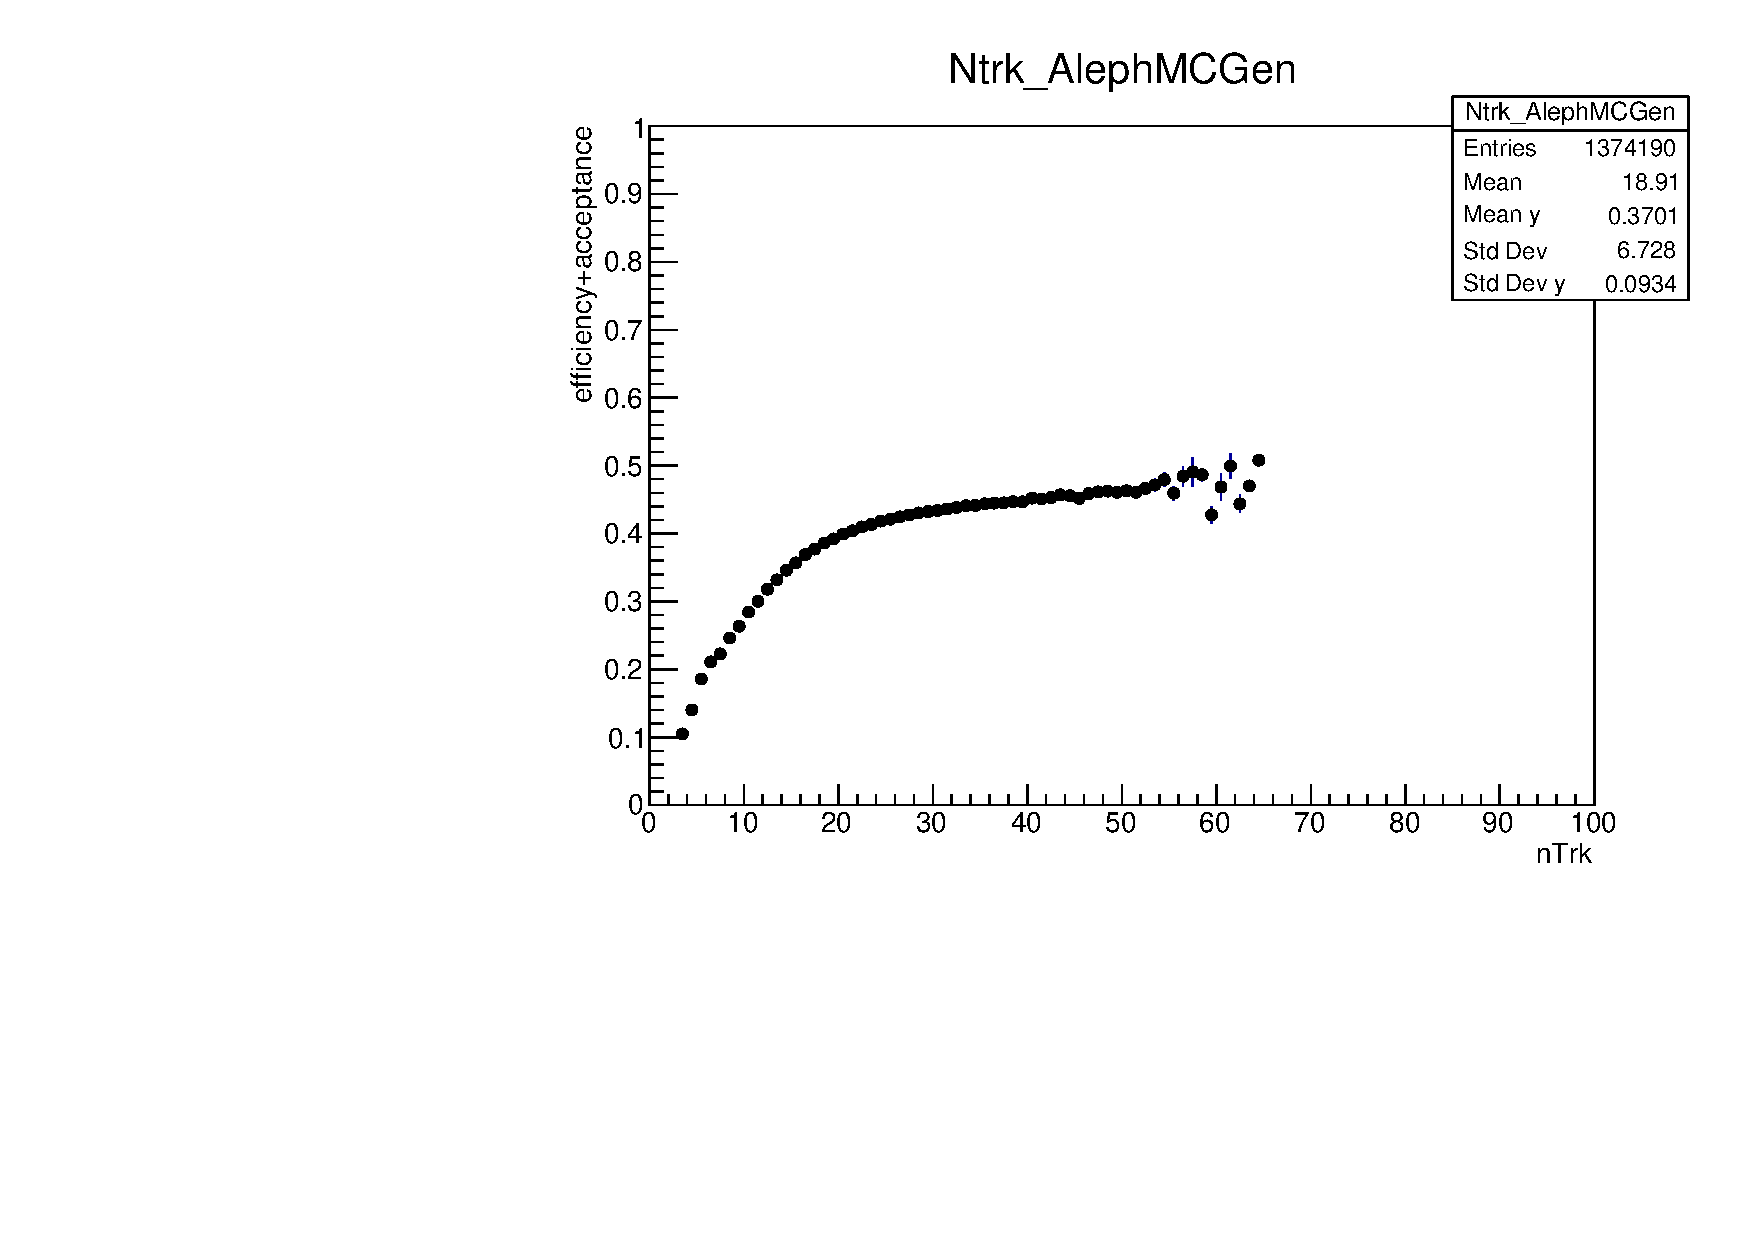
\includegraphics[width=.45\textwidth]{images/MultiplicityConversion/nTrk_AlephMCGen.pdf}
\caption{LEP1 Efficiency+Acceptance Distribution vs Multiplicity}
\label{fig:LEP1EffAccept} 
\end{center}
\end{figure}

\begin{figure}[!htb]
\begin{center}
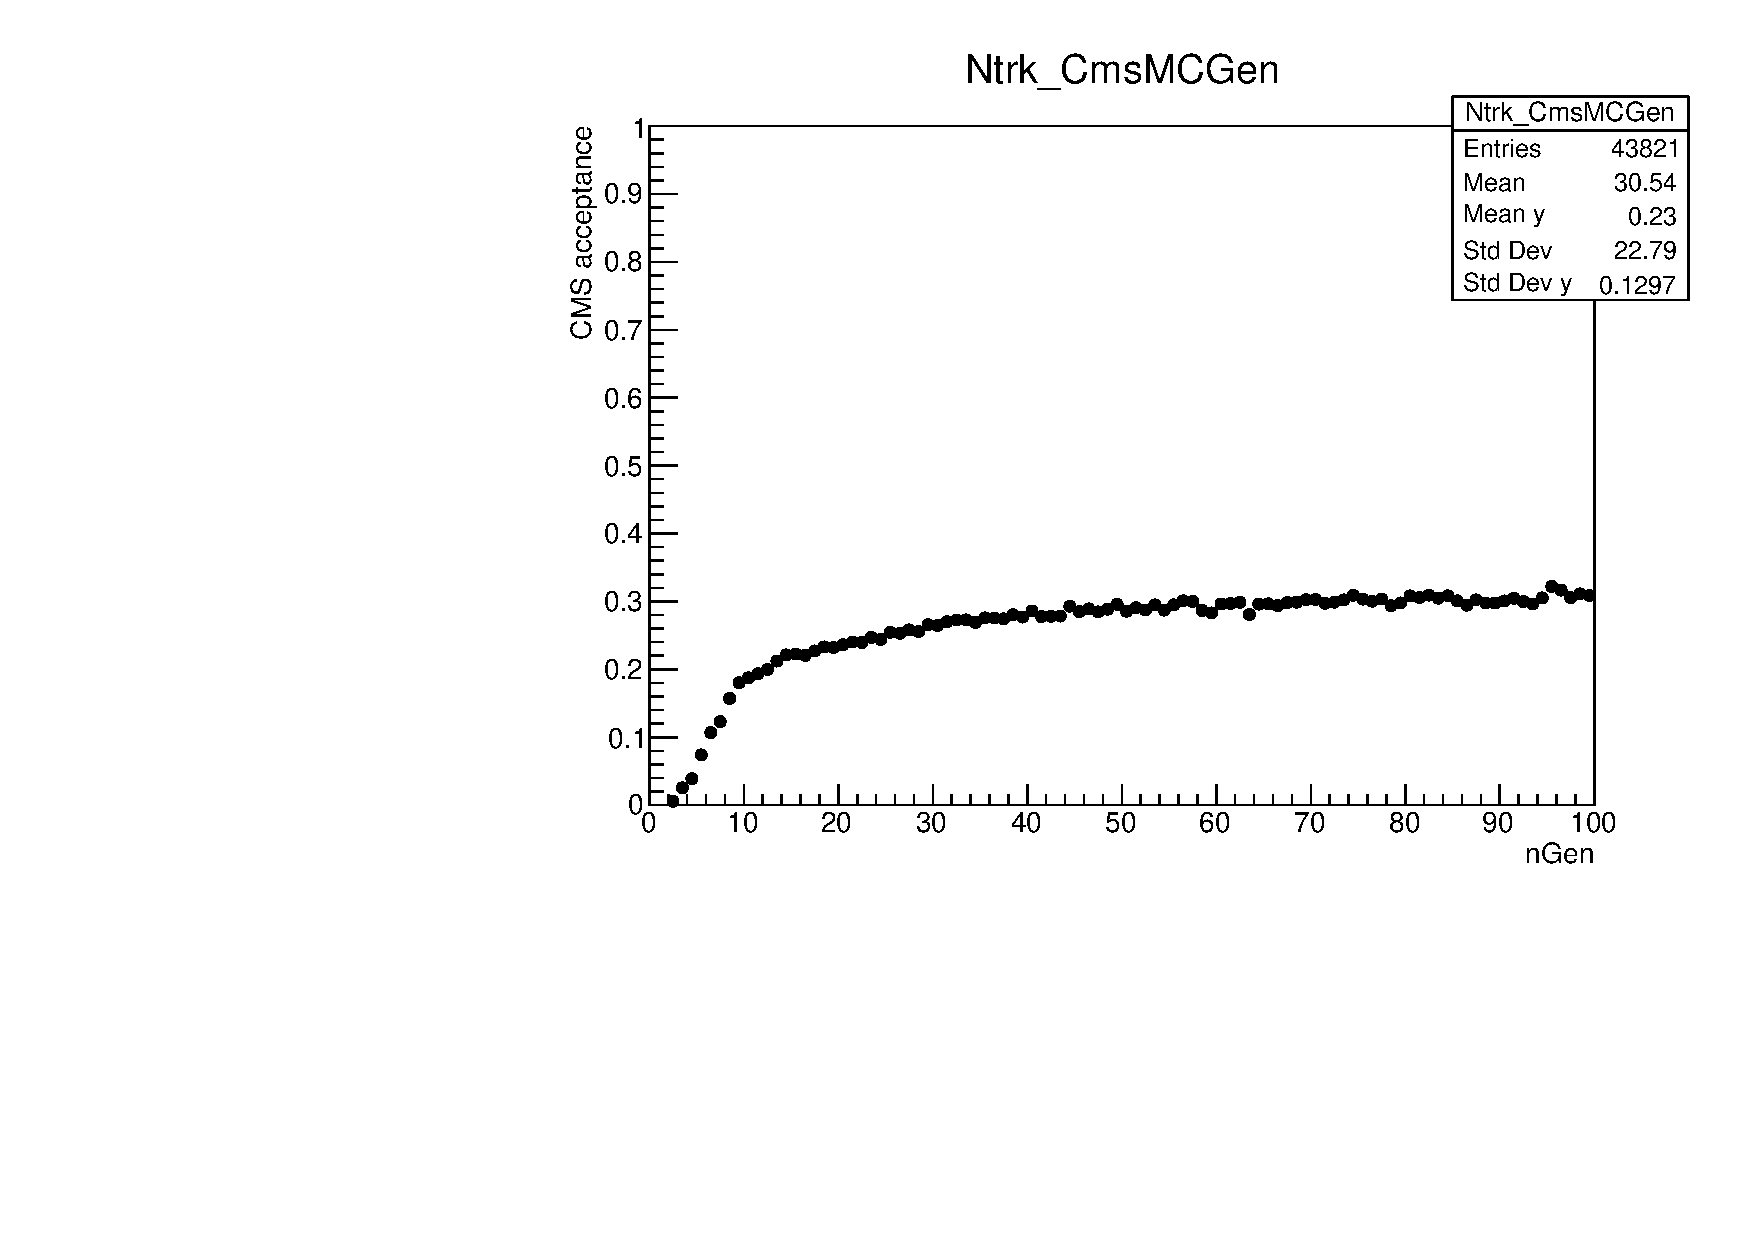
\includegraphics[width=.45\textwidth]{images/MultiplicityConversion/nTrk_CMSMCGen.pdf}
\caption{CMS Acceptance Distribution vs generator-level Multiplicity}
\label{fig:CMSAcc} 
\end{center}
\end{figure}

\begin{figure}[!htb]
\begin{center}
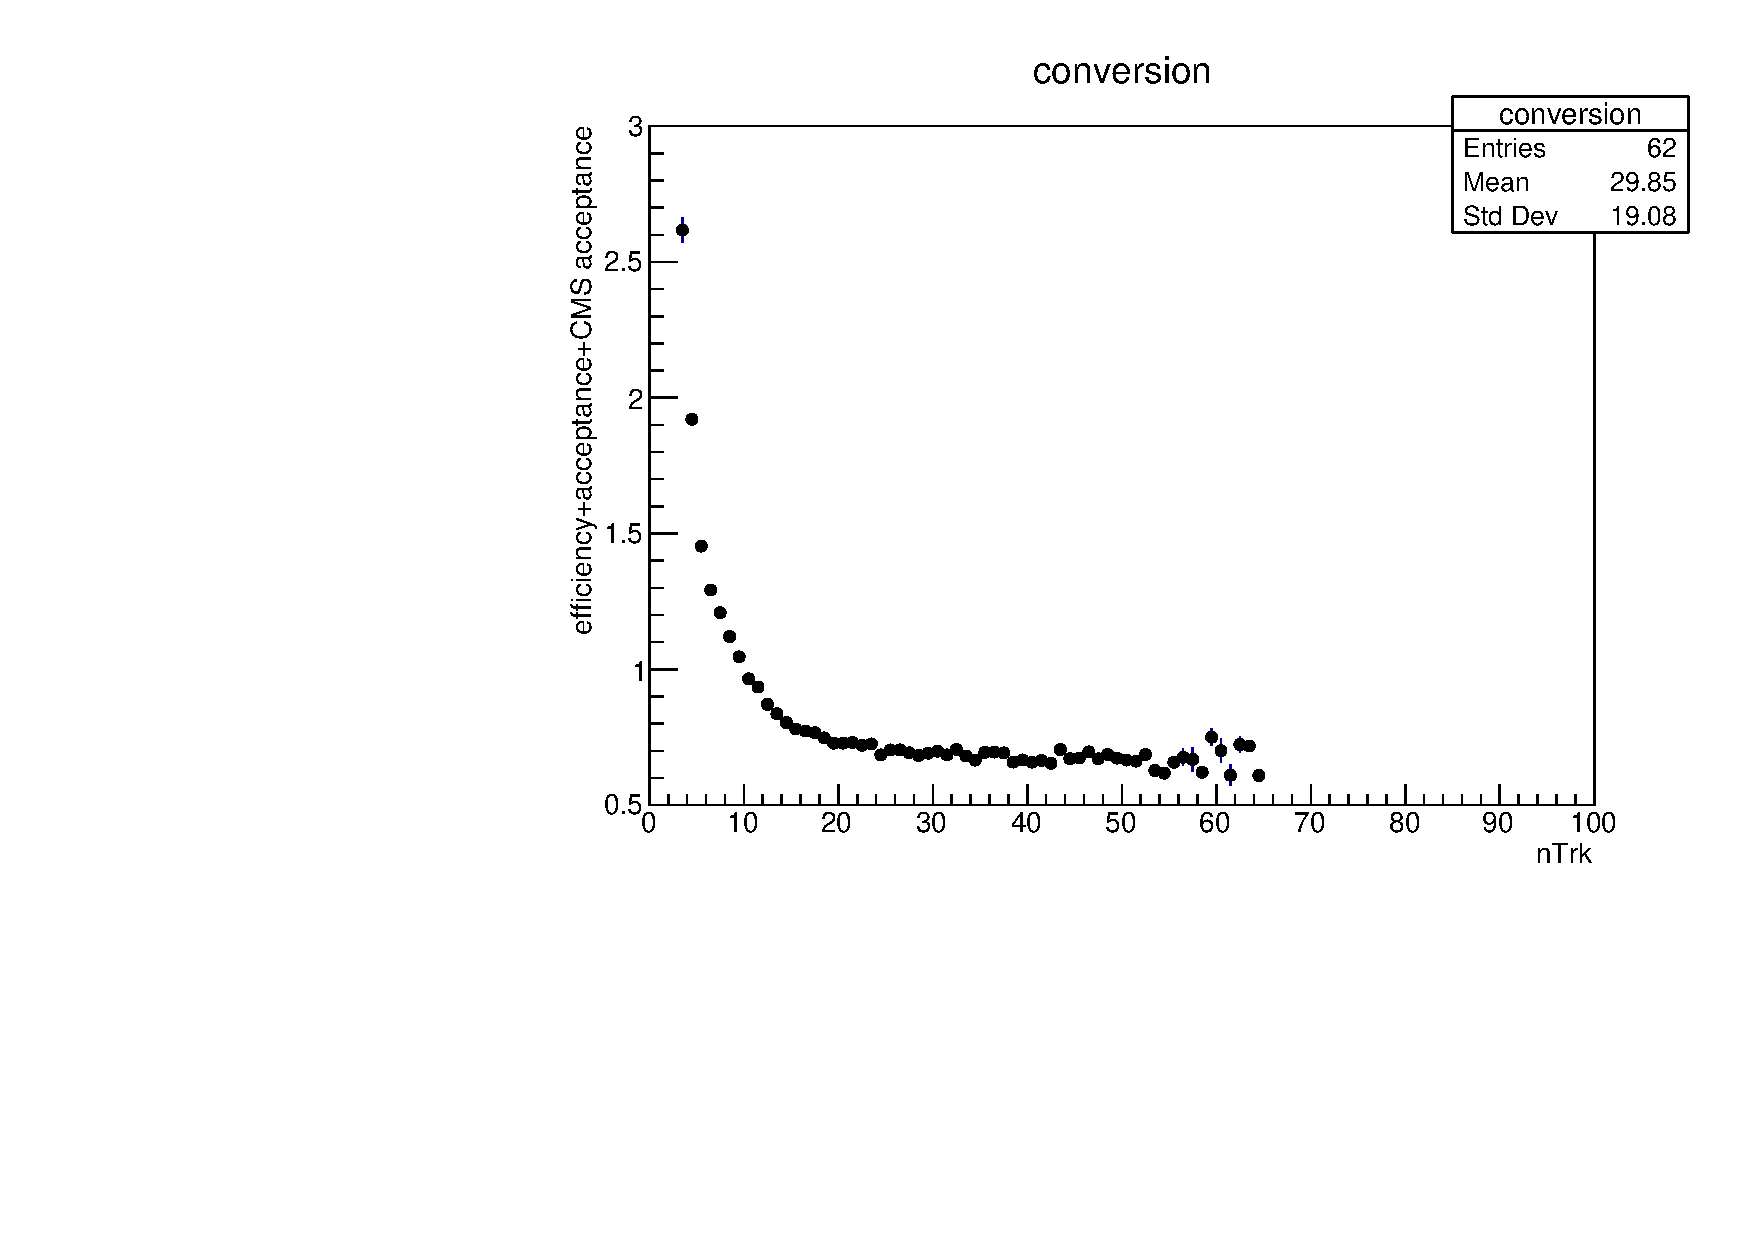
\includegraphics[width=.45\textwidth]{images/MultiplicityConversion/conversion.pdf}
\caption{Conversion factor from ALEPH to CMS multiplcity}
\label{fig:conversion} 
\end{center}
\end{figure}

\begin{figure}[!htb]
\begin{center}
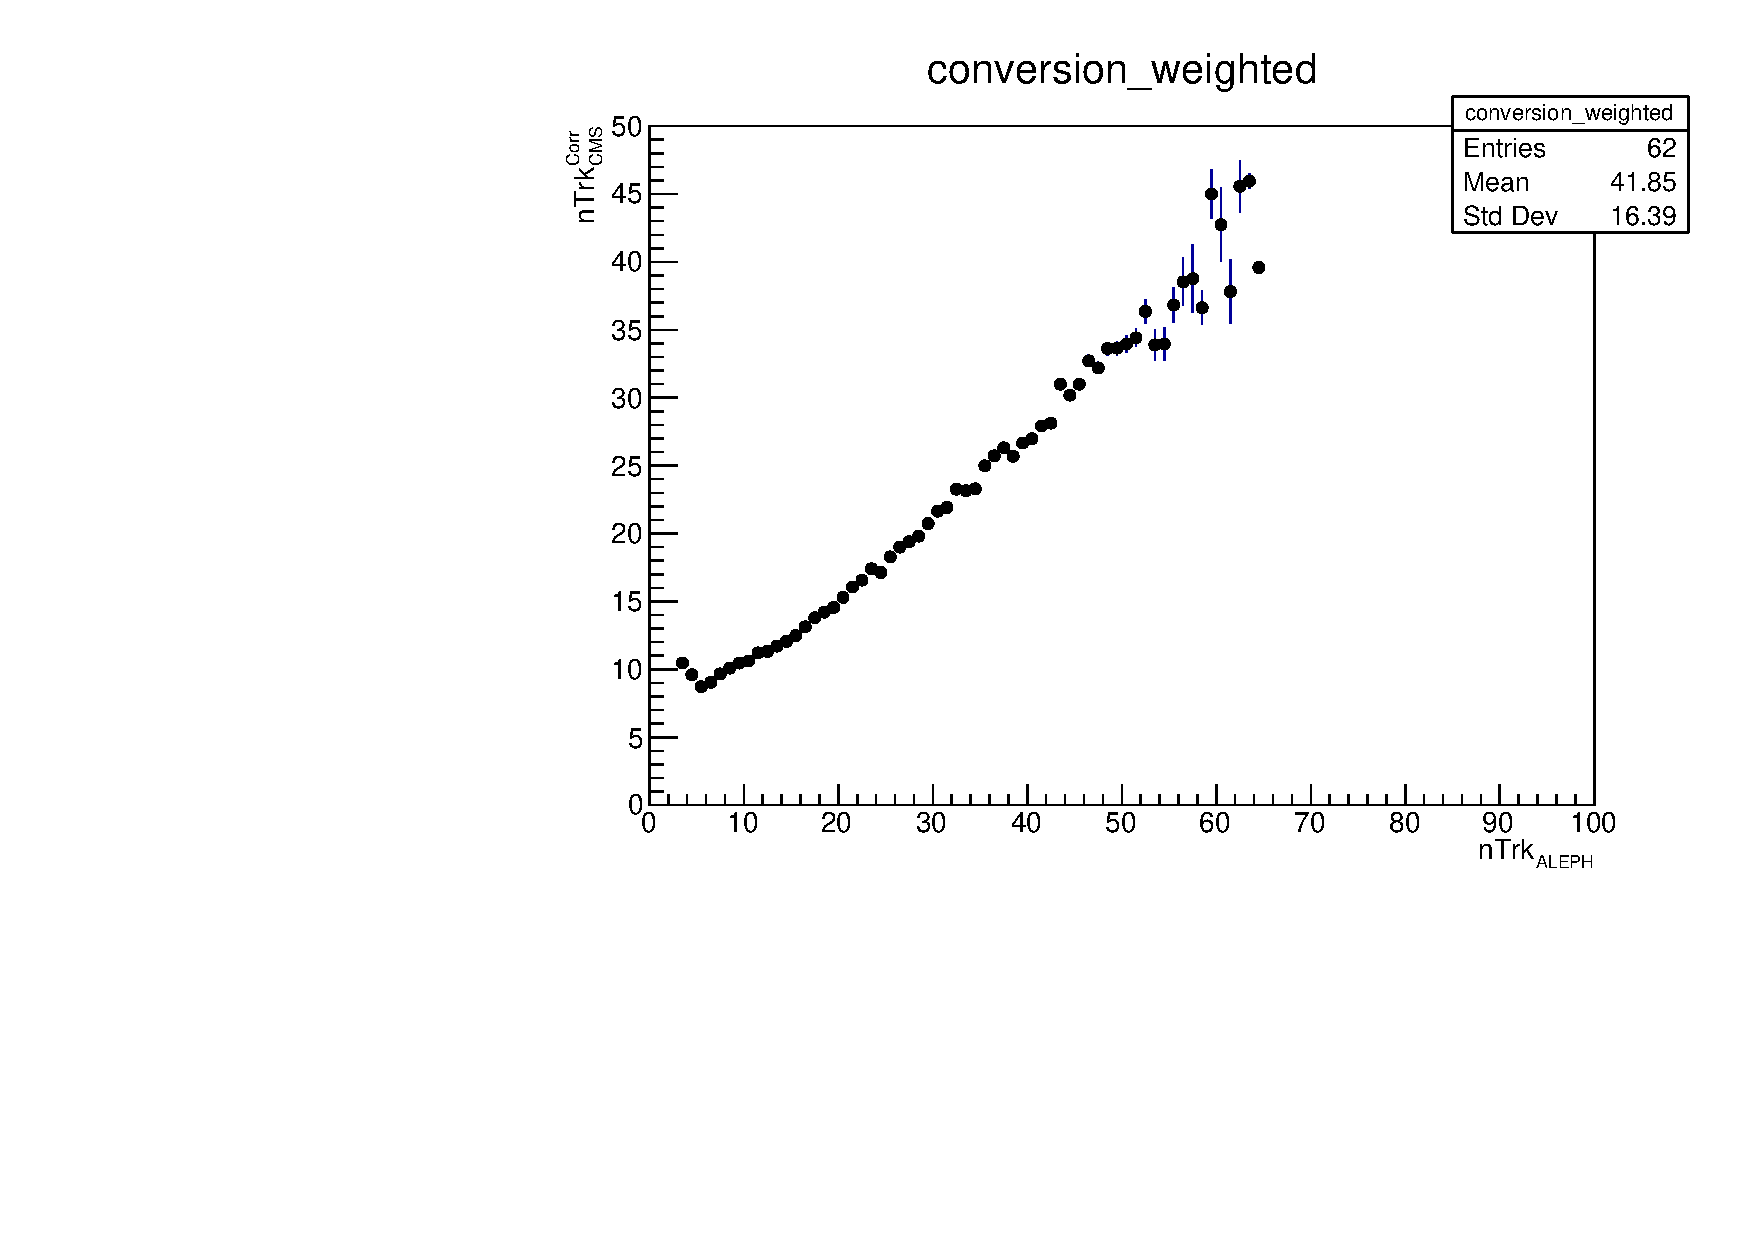
\includegraphics[width=.45\textwidth]{images/MultiplicityConversion/conversion_weighted.pdf}
\caption{Conversion mapping from ALEPH to CMS multiplcity}
\label{fig:conversion2} 
\end{center}
\end{figure}

\begin{figure}[!htb]
\begin{center}
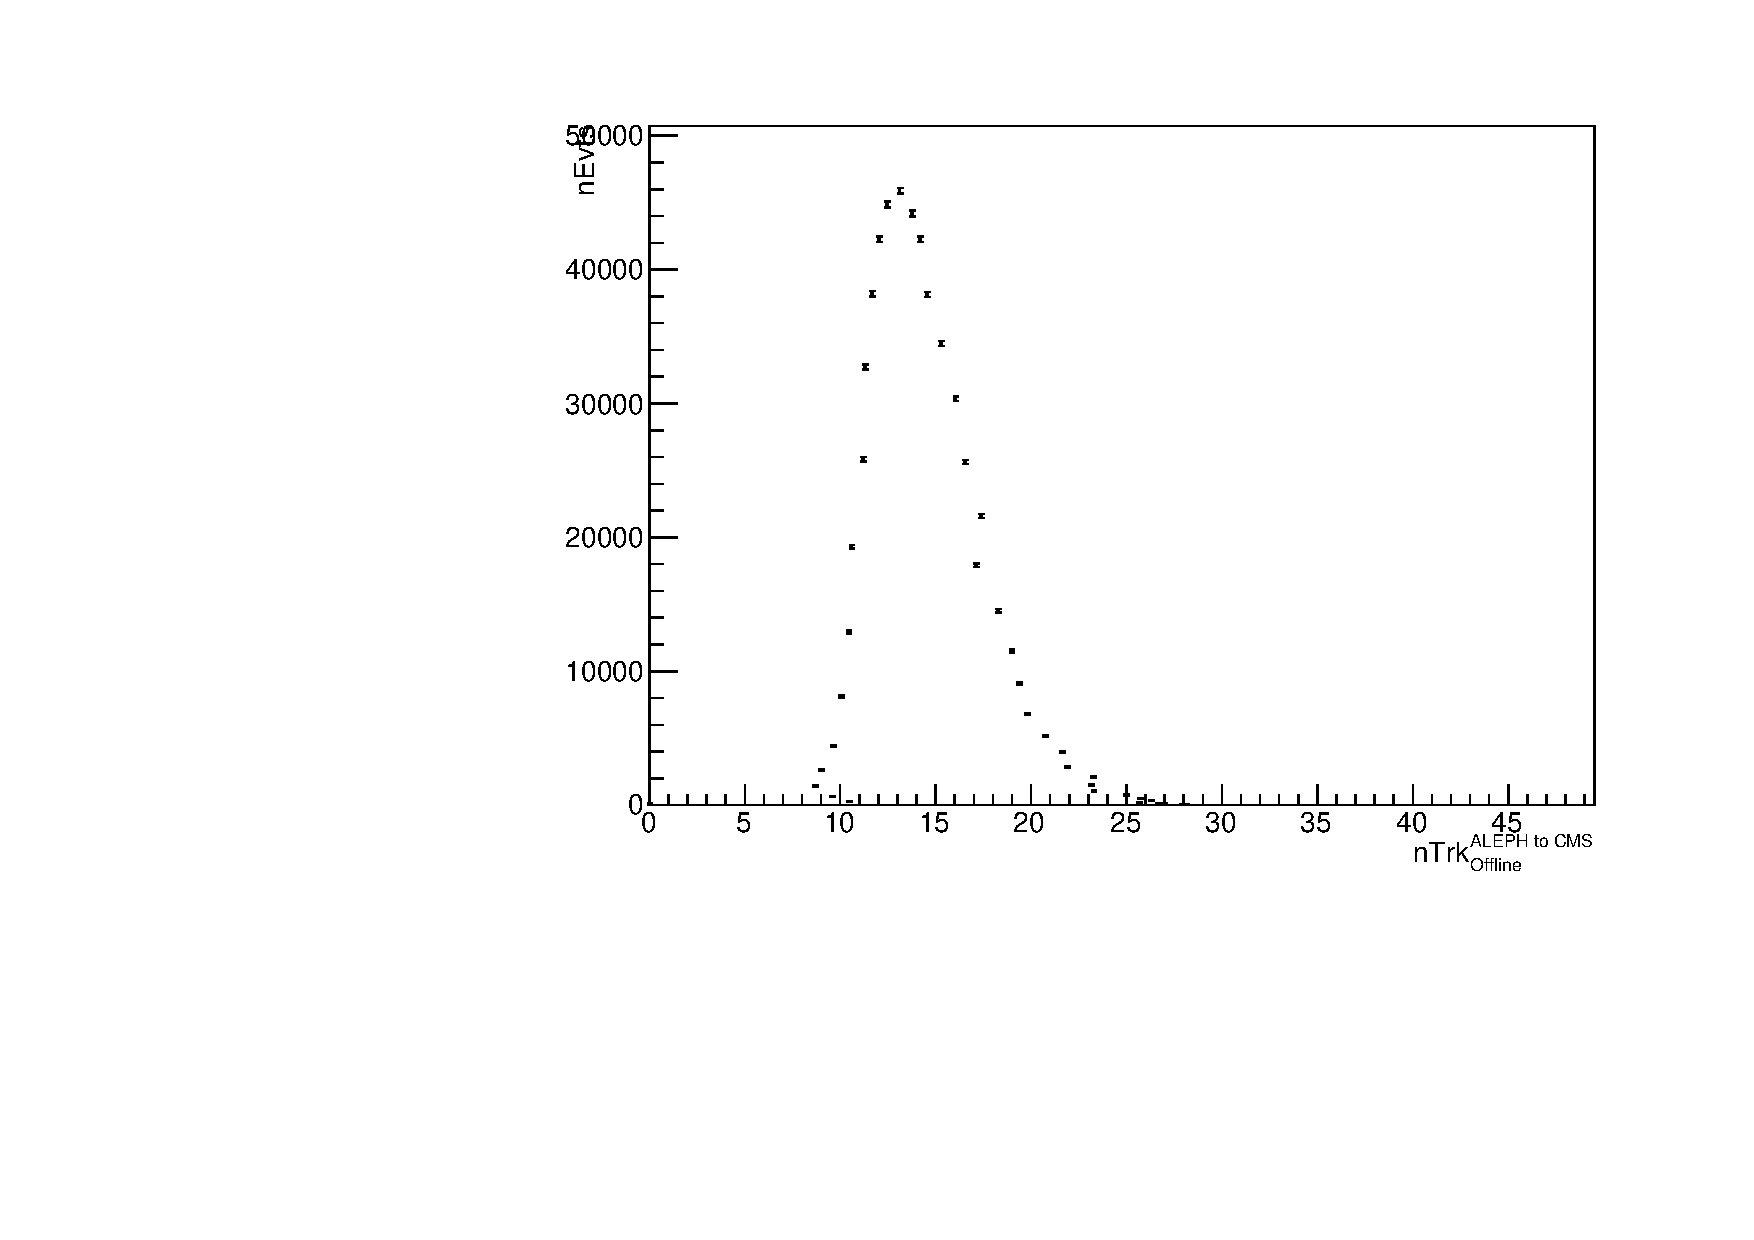
\includegraphics[width=.45\textwidth]{images/MultiplicityConversion/new_nTrk_ALEPHConverted.pdf}
\caption{Scaled ALEPH multiplcity for comparing to CMS}
\label{fig:CMSComparison} 
\end{center}
\end{figure}